%!TEX root = ../Thesis.tex

\chapter{Fahrspur-Bestimmung aus Trajektorie-Clustern}
\label{cha:lane_definition}

In diesem Kapitel wird beschrieben, wie aus den bereits identifizierten Trajektorie-Clustern
Geometrie-Informationen der Fahrspuren abgeleitet werden. Hierzu sind primär drei Schritte notwendig:
Bestimmung der Spur-Mittellinien, Bestimmung der Spurhüllen und anschließend die Partitionierung sich überlagernder
Spuren. Hinzu kommen weitere kleine Schritte, welche ebenfalls nachfolgend beschrieben werden.

\section{Ausfilterung von Spurwechselvorgängen}
\label{sec:real2_filter_lane_change}

Bevor mithilfe der im vorherigen Schritt gewonnenen Trajektorie-Cluster Mittellinien von Fahrspuren bestimmt
werden können, müssen diese nochmals vorverarbeitet werden. Die einzelnen Cluster enthalten teilweise
Bewegungsbahnen, welche Spurwechselvorgänge oder andere Abweichungen von einer Fahrspur beschreiben.
Diese Trajektorien müssen, so weit wie möglich,
entfernt werden, da sie die anschließende Geometrie-Bestimmung negativ beeinträchtigen. Die Trajektorien
eines Clusters sollten eindeutig einer realen Fahrspur zuzuordnen sein. In Abbildung
\ref{fig:real2_clusters_pre_postpro} sind beispielhaft zwei Cluster dargestellt, welche eine Vielzahl an
Spurwechselvorgängen enthalten.

\begin{figure}[H]
    \centering
    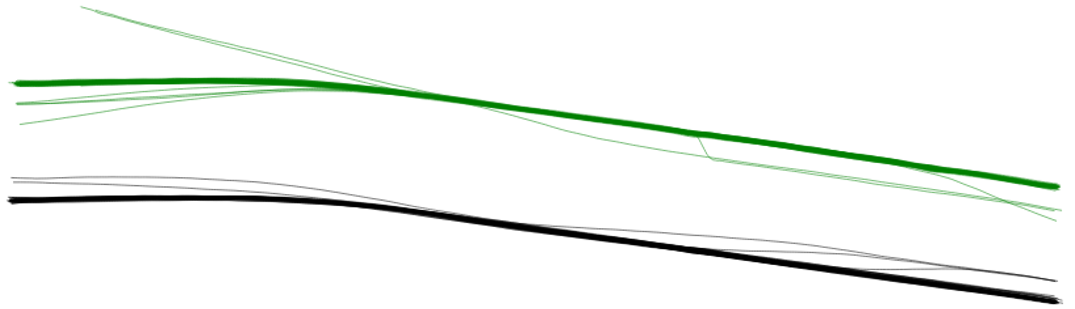
\includegraphics[width=0.8\linewidth]{resources/img/umsetzung/U2/Clusters_Pre_Postprocessing}
    \caption{Trajektorie-Cluster mit Spurwechselvorgängen}
    \label{fig:real2_clusters_pre_postpro}
\end{figure}

Die Grundidee, welche der Ausfilterung der Abweichungen zugrunde liegt, ist, jene Trajektorien
aus einem Cluster zu entfernen, welche eine überdurchschnittlich hohe mittlere Distanz zu allen anderen
Trajektorien des Clusters besitzen. Als Distanzmaß wird erneut die LCSS Distanz verwendet.
Ein ähnlicher, Distanz-basierter Ausreißer-Detektionsansatz wird in \cite[]{Mirge2017} vorgestellt.
Der in dieser Arbeit verwendete Algorithmus ist in Listing \ref{lst:pseudo_post_processing} beschrieben.

\begin{lstlisting}[caption=Pseudocode Cluster Post-Processing, language=Pseudo, label=lst:pseudo_post_processing]
algorithm filterCluster:
  input:  unfiltered trajectories of cluster: trajsIn
  output: filtered trajectories of cluster

  meanTrajectoryDistances :=
    for each traj in trajsIn do
      yield mean LCSS distance of traj to all other trajectories of trajsIn
    end

  clusterCmpVal := select median of meanTrajectoryDistances as comparison value

  resultTrajs :=
    for each traj in trajsIn do
      if meanDist of traj < 1.5 * clusterCmpVal then
        yield trajs
      end
    end

  return resultTrajs
\end{lstlisting}

Das gewählte Verfahren ist einfach, eignet sich aber dennoch gut, um das gewünschte Ziel zu erreichen.
Die in Abbildung \ref{fig:real2_clusters_post_postpro} dargestellten Ergebnisse zeigen dies.
Aus den in Abbildung \ref{fig:real2_clusters_pre_postpro} enthaltenen Clustern wurden alle Trajektorien
mit Spurwechselvorgängen oder Abweichungen entfernt. Die Effektivität konnte auch durch die Anwendung
auf andere Datensätze bestätigt werden.
Wenn in einem Cluster viele Trajektorien Abweichungen von einer Spur besitzen, ist es möglich, dass der Algorithmus
diese nicht vollständig entfernt. Bei einer geringen Anzahl von Abweichungen oder Ausreißer arbeitet
er allerdings sehr zuverlässig.

\begin{figure}[H]
    \centering
    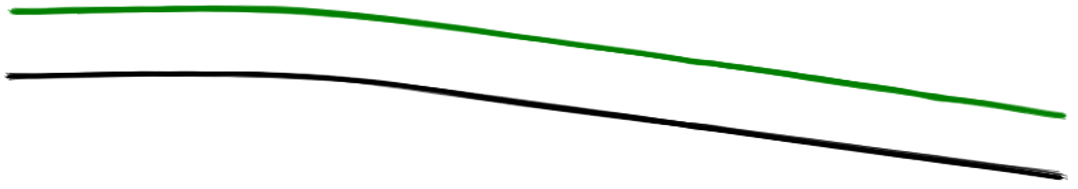
\includegraphics[width=0.8\linewidth]{resources/img/umsetzung/U2/Clusters_Post_Postprocessing}
    \caption{Trajektorie-Cluster ohne Spurwechselvorgänge}
    \label{fig:real2_clusters_post_postpro}
\end{figure}

Zu beachten ist allerdings auch, dass die Zeitkomplexität des Verfahrens bei großen Trajektorie-Clustern
nicht unerheblich ist. Dies ist auf die Komplexität des LCSS Distanzmaßes zurückzuführen.
Bei der Untersuchung alternativer Vorgehensweise wurde allerdings klar, dass es grundlegend schwer ist,
das Problem der Ausreißer-Erkennung performant zu lösen.
In \cite[]{Meng2018} werden hierzu diverse Distanz- und Dichte-basierte
Arbeiten vorgestellt und verglichen. Da diese alle allerdings nicht weniger komplex sind und häufig
die verfolgten Ziele über die hier geforderten hinausgehen, wurde entschieden den oben beschriebenen Ansatz
beizubehalten. Durch die Parallelisierung der Berechnung der mittleren Abstände konnte die Performance
des Ansatzes außerdem nochmals deutlich gesteigert werden.

\section{Bestimmung der Spurmittellinien}
\label{sec:real2_define_lane_centerline}

Nachdem die Trajektorie-Cluster nun weitestgehend von Fahrspurwechseln und anderen Abweichungen bereinigt
wurden, beschreiben die verbleibenden Bewegungsbahnen eines Clusters eine Fahrspur.
Anhand dieser Trajektorien können daher nun die Mittellinie der Spuren bestimmt werden.

Die zu bestimmende Mittellinie verläuft durch die Mitte des entsprechenden
Trajektorie-Clusters. Die einzelnen Bewegungsbahnen besitzen jeweils leichte Abweichungen von dieser
\textit{``Ideallinie''}.
Als Spurmittellinie -- wie von \cite{Hu2005} vorgeschlagen -- jene Trajektorie zu wählen, welche die
kleinste Summe der Distanzen zu allen anderen Trajektorien eines Clusters besitzt, ist nicht praktikabel,
da die so gefunden Trajektorie nicht über ihre komplette Länge in der Mitte des Clusters verlaufen muss.
Auf eine Bestimmung der Mittellinie mittels linearer oder polynomialer Regression, wie beispielsweise in
\cite[]{Chen2014} oder \cite[]{Melo2006},
wurde ebenfalls verzichtet. Der Grund hierfür ist, dass einerseits die Komplexität und Form der Fahrbahnverläufe
nicht bekannt ist und andererseits das Erlernen der Spurrepräsentation zu aufwendig ist.

Der in dieser Arbeit gewählte Ansatz zur Bestimmung der Spurmittellinien macht sich die von Atev et al.
vorgestellte Notation einer relativen Position innerhalb einer Trajektorie zu nutze, welche in
Gleichung \ref{eq_atev_relPos} und \ref{eq_atev_findPointAtRelPow} gegeben ist.
Die Koordinaten der Spurlinien ergeben sich aus den Mittelwerten von Trajektorie-Punkten, welche sich
alle an der selben relativen Position befinden. Der verwendete Algorithmus ist nachfolgend beschrieben.
\begin{lstlisting}[caption=Pseudocode Cluster Post-Processing, language=Pseudo, label=lst:pseudo_post_processing]
algorithm calculateCenterline:
  input:  trajectories of cluster: trajsIn
  output: centerline of lane

  meanTrajLength := calculate mean point length of trajectories
  relPositions := define range with relative positions of size meanTrajLength
                  and step-size (1 / meanTrajLength)

  centerline :=
    for each relP in relPositions do
      pointsAtRelPos := get points at relP for each traj in trajsIn
      yield mean of all points in pointsAtRelPos
    end

  return centerline
\end{lstlisting}
% TODO: keywords escapen

Da die Form und der Verlauf von Trajektorien eines Clusters sich nur wenig unterscheiden, liefert dieses
Vorgehen gute Ergebnisse. In Abbildung \ref{fig:real2_results_centerline_detection} a) ist beispielhaft
dargestellt, wie eine Mittellinien innerhalb eines Trajektorie-Clusters verlaufen.
In \ref{fig:real2_results_centerline_detection} b) sind alle Spurmittellinien der Neckartor-Kreuzung,
welche auf die oben beschriebene Weise bestimmt wurden, abgebildet.

% TODO: Bild mit Spurmittellinien in Aufnahme
\begin{figure}[H]
    \centering
    \subfloat[]{{
        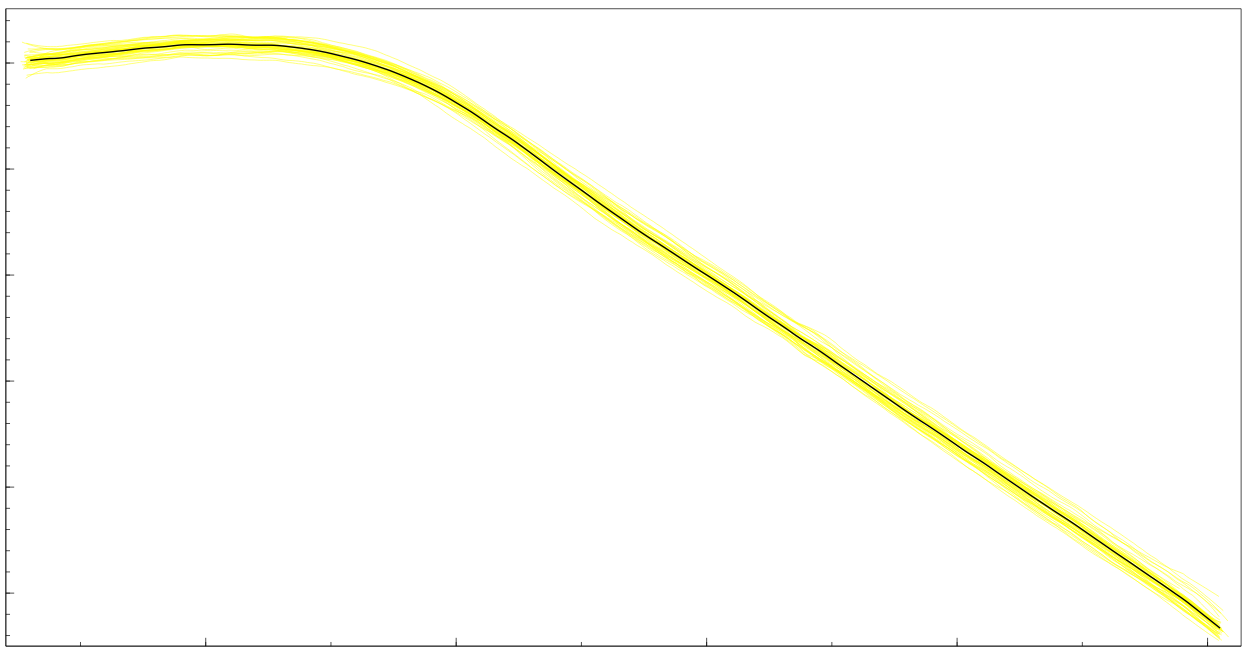
\includegraphics[align=c, width=0.45\linewidth]{resources/img/umsetzung/U2/cluster_with_centerline}
    }}
    \qquad
    \subfloat[]{{
        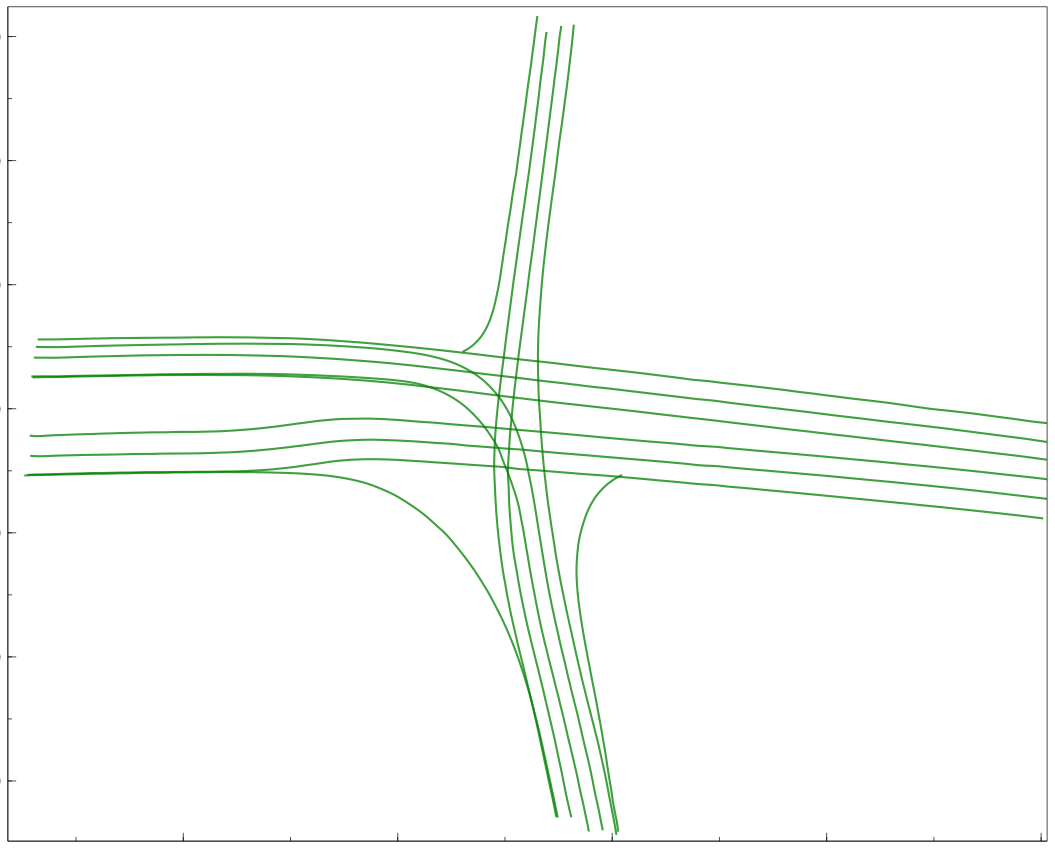
\includegraphics[align=c, width=0.4\linewidth]{resources/img/umsetzung/U2/laneCenters}
    }}
    \caption{Spurmittellinie in einem Trajektorie-Cluster a), Spurmittellinien Neckartor-Kreuzung b)}
    \label{fig:real2_results_centerline_detection}
\end{figure}

Die Mittellinien werden, da es sich bei ihnen ebenfalls um Sequenzen von 2D-Koordinaten handelt,
über Trajektorie-Objekte repräsentiert (siehe Abbildung \ref{fig:real_trajectory_classDia}).

\section{Angleichung benachbarter Spur-Enden}
% Grund hierfür (Besser für Analyse)
% Bild vor und nach der Angleichung
% Beschreibung Vorgehen
    % Suche benachbarter Spurenden
    % Bestimmung der am weitesten ausstehenden Spur
    % orthogonal-projektion der anderen benachbarten Spuren auf Höhe der äußersten

Bevor für jede Spurmittellinie eine Hülle definiert wird, welche die Geometrie der Fahrspur definiert,
werden benachbarte Spur-Enden aneinander angeglichen. Diese sollen immer auf der selben Höhe beginnen
beziehungsweise enden, um sie beispielsweise bei der Spurwechsel-Analyse besser vergleichen zu können.

Benachbarte Fahrspuren können einen deutlich sichtbaren Versatz an ihren Anfängen
und Enden besitzen, was beispielsweise in Abbildung \ref{fig:real2_lane_alignment} a) dargestellt ist. Diese Unterschiede entstehen
primär, da Fahrzeuge am Rand der Aufnahme verschieden schnell erkannt werden und so deren Trajektorien
unterschiedlich früh beginnen. Für das Angleichen der Spur-Enden sind grundlegend drei Schritte notwendig:
Finden von benachbarten Enden, Bestimmung der längsten Spur im Bereich der Enden und schließlich das
Angleichen aller Spuren auf die Höhe der vorher bestimmten ``äußersten'' Mittellinie.

Gruppen benachbarter Spur-Enden werden auf rekursive Weise gefunden. Es wird eine Spur gewählt und im
Bereich ihres Starts beziehungsweise Endes nach unmittelbaren Nachbarn gesucht. Das hierzu verwendete
Verfahren ist in Abschnitt \ref{sec:real2_identify_parallel_lanes} beschrieben. Für jede der so gefundenen
Nachbarspuren wird wiederum nach deren Nachbarn gesucht. Auf diese Weise ergibt sich eine Spur-Gruppe.

Da das Weltkoordinaten-System in den verwendeten Aufnahmen keine feste Orientierung und keinen fixen Ursprung besitzt,
kann die in einer Spur-Gruppe am weitesten außen liegende Spur nicht identifiziert werden, indem die
Koordinaten der Start- oder Endpunkte der Spuren verglichen werden.
Bestimmt wird die ``äußerste'' Mittellinie daher, indem durch jeden Endpunkt der Spuren einer Gruppe
eine orthogonale Gerade gelegt wird. Die Spur deren zugehörige orthogonale Gerade die wenigsten Schnittpunkte
mit anderen Spur-Mittellinien besitzt, liegt am weitesten außen. Abbildung \ref{fig:real2_lane_alignment_concept}
veranschaulicht das Vorgehen.

\begin{figure}[H]
    \centering
    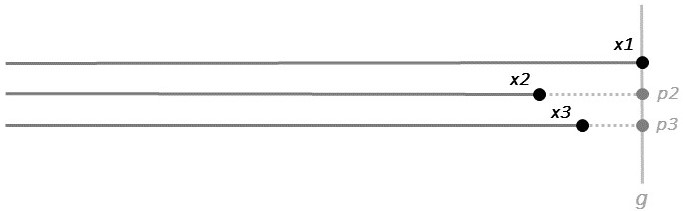
\includegraphics[width=0.5\linewidth]{resources/img/umsetzung/U2/LaneAlignment_concept}
    \caption{Konzept der Spur-Enden-Angleichung}
    \label{fig:real2_lane_alignment_concept}
\end{figure}

Die so bestimmte Gerade $g$ ist zudem gleichzeitig, die Linie, auf welche die anderen Spur-Endpunkte
projiziert werden. Hierzu wird eine Orthogonalprojektion der Endpunkte auf die Gerade $g$ durchgeführt, welche
in Gleichung \ref{eq_orthPro} definiert ist. $\vec r_0$ entspricht hierbei einem Stützvektor auf der Geraden $g$ und
$\vec u$ dem Richtungsvektor.

\begin{ceqn}
\begin{align}
\label{eq_orthPro}
    P_g(\vec x) =  \vec r_0 + \frac{( \vec x - \vec r_0 ) \cdot \vec u}{\vec u \cdot \vec u} \, \vec u
\end{align}
\end{ceqn}

Das Ergebnis der Spur-Angleichung ist in Abbildung \ref{fig:real2_lane_alignment} b) dargestellt.

\begin{figure}[H]
    \centering
    \subfloat[]{{
        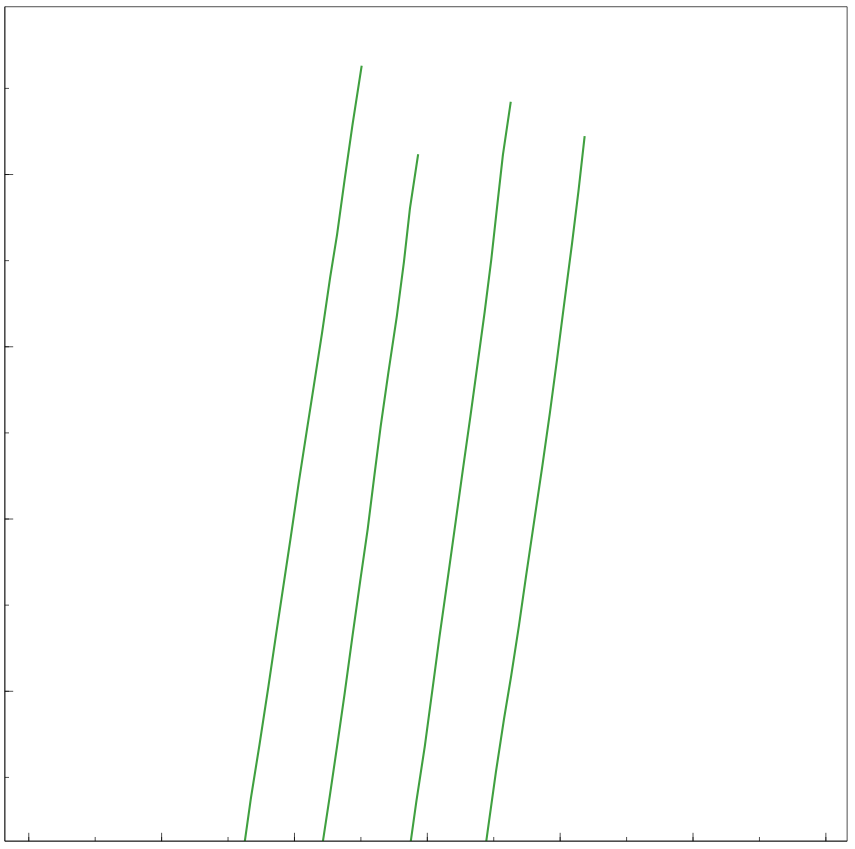
\includegraphics[align=c, width=0.25\linewidth]{resources/img/umsetzung/U2/normalCenterLines}
    }}
    \qquad \qquad
    \subfloat[]{{
        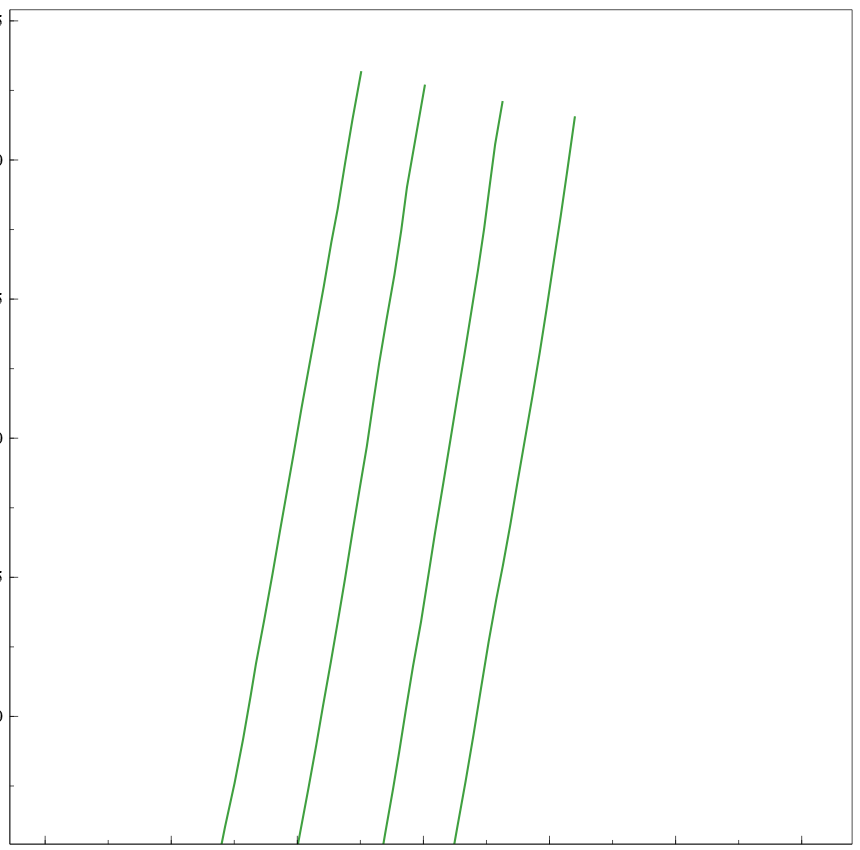
\includegraphics[align=c, width=0.25\linewidth]{resources/img/umsetzung/U2/alignedCenterLines}
    }}
    \caption{Mittellinien ohne Angleichung a) und mit Angleichung b)}
    \label{fig:real2_lane_alignment}
\end{figure}

Nachdem die Spurmittellinien auf die oben beschriebene Weise angeglichen wurden, werden anschließend
Spurhüllen definiert.

\section{Bestimmung der Spurhüllen}
\label{sec:real2_define_lane_envelope}

Nachdem die Mittellinien der Fahrspuren bestimmt und ihre Enden aneinander angeglichen wurden, wird nun für jede Spurlinie
eine Hülle definiert. In folgendem Abschnitt wird beschrieben, wie diese erstellt werden.

Die Spurhülle bestimmt die Dimension einer Fahrbahn. In dieser Arbeit verlaufen sie idealerweise entlang
realer Begrenzungslinien welche zwei Spuren voneinander oder eine Fahrbahn von einem Seitenstreifen et cetera trennen.
Eine Mittellinie und eine Hülle beschreiben zusammen die Geometrie einer Fahrspur. Diese Geometrie
soll die realen Dimensionen einer Spur möglichst genau abbilden. Aus diesem Grund ist es nicht möglich,
die Hüllen lediglich auf Basis von statistischen Informationen der Trajektorie-Cluster zu bestimmen,
wie das beispielsweise in \cite[]{WeimingHu2006} oder \cite[]{Morris2011} gemacht wird.
Der in dieser Arbeit verwendete Ansatz zur Bestimmung der Spurhüllen basiert daher lediglich auf den
Spurmittellinien und nutzt ihre relative Lage zueinander. Ansätze hierzu stammen aus den Arbeiten von
\cite[]{Hsieh2006} und \cite[]{Makris2005}, welche in Abschnitt \ref{sec:rw_lane_detection} vorgestellt wurden.

Die grundlegende Idee, auf welcher die Bestimmung der Spurhüllen basiert, ist konzeptionell in Abbildung
\ref{fig:real2_envelope_definition_concept} dargestellt.
Für zwei parallel zueinander verlaufende Spuren $l_1$ und $l_2$ werden die Hüllen über den Abstand zwischen
ihren Mittellinien bestimmt. Besitzen die Linien den Abstand $d$ zueinander, so beträgt die Breite
der Spuren ebenfalls $d$. Der Abstand $e_d$ zwischen einer Mittellinie und einer Hüll-Linie beträgt folglich
$1/2\ d$.

\begin{figure}[H]
    \centering
    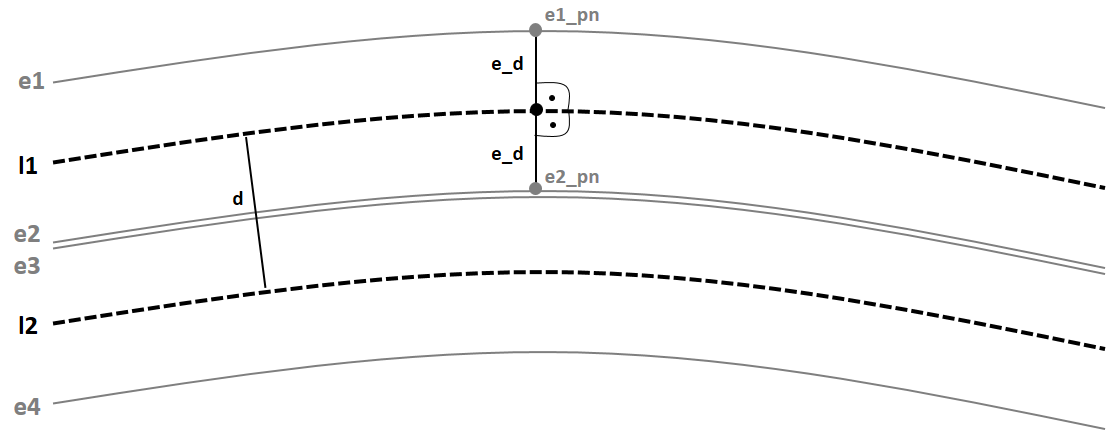
\includegraphics[width=0.75\linewidth]{resources/img/umsetzung/U2/concept_lane_envelope}
    \caption{Bestimmung Spürhüllen}
    \label{fig:real2_envelope_definition_concept}
\end{figure}

Die oben beschriebene Definition einer Bahn-Geometrie wird im Spurerkennungs-Modul über eine Klasse
\textit{LaneGeometry} repräsentiert. Diese ist in Abbildung \ref{fig:real2_laneGeometry_ClassDia} dargestellt.
Das Feld \textit{variance} entspricht dem Abstand $e_d$ zwischen der \textit{centerline} und den Hüll-Linien.

\begin{figure}[H]
    \centering
    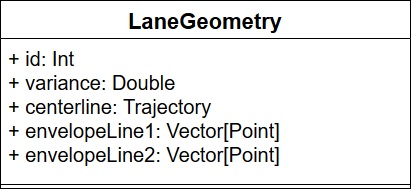
\includegraphics[width=0.38\linewidth]{resources/img/umsetzung/U2/LaneGeometry_ClassDia}
    \caption{Aufbau LaneGeometry Klasse}
    \label{fig:real2_laneGeometry_ClassDia}
\end{figure}

Einen ähnlichen Ansatz zur Bestimmung von Spurbegrenzungslinien verwenden auch Hsieh et al. in ihrer Arbeit.
Sie gehen jedoch, da die von ihnen verwendeten
Aufnahmen von einer statischen Kamera über einer Autobahn stammen, davon aus, dass alle Fahrspuren parallel
zueinander verlaufen. Da das in dieser Arbeit entwickelte Spurerkennungs-Modul mit unterschiedlichen
Aufnahmen und Straßentopologien umgehen können muss, kann diese Annahme nicht getroffen werden.
Nachfolgend werden die Schritte vorgestellt, welche angewandt werden, um in einer Menge von Spuren
jene zu finden, welche parallel zueinander verlaufen. Auf deren Basis werden anschließend die Spurbreiten bestimmt und
die Hüll-Linien definiert.

\subsection*{Identifikation paralleler Fahrspuren}
\label{sec:real2_identify_parallel_lanes}

Um in einer Menge von Fahrspuren, welche über Mittellinien repräsentiert werden, jene zu finden, die
parallel zueinander verlaufen, werden in einem ersten Schritt benachbarte Spur-Paare gesucht.
Zwei Fahrspuren $l1$ und $l2$ gelten als benachbart, wenn sich der Start oder das Ende
von Spur $l2$ in einem Bereich mit Radius $\sigma$ um den Start von $l1$ befindet.
Der Wert für $\sigma$ wurde auf Basis der in Deutschland geltenden
\textit{``Richtlinien für die Anlage von Autobahnen''} (\acrshort*{raa}) \cite[]{RAA2008}
und der \textit{``Richtlinien für die Anlage von Landstraßen''} (\acrshort*{ral}) \cite[]{RAL2012} bestimmt. Diese Regelwerke spezifizieren
die in der Bundesrepublik derzeit zulässigen Straßenquerschnitte. Die in ihnen festgelegten
Spurbreiten variieren zwischen 3.25 und 3.75 Metern.
Um auch besonders breite benachbarte Spur-Paare identifizieren zu können, wurde für $\sigma$ der Wert 4m gewählt.

Die auf diese Weise gefundenen Trajektorie-Paare starten oder enden als benachbarte Spuren.
Der Algorithmus welcher prüft, ob zwei Spuren tatsächlich parallel zueinander verlaufen, ist in Listing
\ref{lst:pseudo_checkParallel} beschrieben. Die zu vergleichenden Mittellinien werden jeweils in eine
Reihe von Richtungsvektoren umgewandelt. Anschließend werden paarweise die Winkel zwischen zwei Vektoren
berechnet und gemittelt.
Liegt die sich so ergebende Abweichung unter einem Grenzwert $\delta$, so handelt es sich um parallele Spuren.
Zusätzlich wird geprüft, ob die Spuren eine ähnliche Länge besitzen.
\begin{lstlisting}[caption=Pseudocode Überprüfung der Parallelität zweier Mittellinien, language=Pseudo, label=lst:pseudo_checkParallel]
algorithm lanesAreParallel:
  input:  lane-centerline: l1, lane-centerline: l2, delta
  output: True or False

  inOppositeDirections := check if l1 and l2 run in opposite directions
  if inOppositeDirections then
    reverse points of centerline l2
  end

  l1DirectionVec := calculate direction vectors for l1
  l2DirectionVec := calculate direction vectors for l2
  dirDifferences := calculate pairwise the angle between two direction vectors

  meanDiff := calculate mean angle of deviation between l1 and l2
  lengthDiff := calculate difference between length of l1 and l2

  return meanDiff < delta && lengthDiff >= 0.8
\end{lstlisting}

Für $\delta$ wurde experimentell der Wert 0.1 bestimmt. In den verschiedenen Test-Datensätzen konnten
so zuverlässig parallele Spur-Paare identifiziert werden. Anhand dieser werden im nächsten Schritt
die Spurhüllen bestimmt.

\subsection*{Berechnung der Hüllen}
\label{sec:real2_create_envelopes}

% Bestimmung der mittleren Distanzen zwischen Spuren, Berechnung der Spurvarianz
% Spuren ohne Nachbar erhalten standard-Varianz
% Berechnung der Hüllen, Formeln, Referenz auf Abb. oben

Bevor für eine Mittellinie die sie umgebende Spurhülle bestimmt werden kann, muss die Breite der Spur
ermittelt werden. Diese ergibt sich, für die im vorherigen Schritt bestimmten parallelen Spurpaare, aus
deren mittleren Abstand zueinander. Verlaufen zu einer Spurlinie zwei Bahnen parallel, werden
die Abstände zu beiden berechnet und der kleinere wird als Spurbreite gewählt.
Allen Bahnen, welche keine parallele Nachbarspur besitzen, wird das Minimum der im vorherigen Schritt bestimmten
Spurbreiten zugeordnet.
Falls sich in einer Aufnahme keine parallelen Spuren befinden, wird für die Spurbreite ein Standartwert
von 3.5 Metern verwendet, welcher sich ebenfalls aus den RAA und RAL Richtlinien ableitet.

Nachdem auf die oben beschriebene Weise Breiten für alle Fahrspuren bestimmt wurden, können die Hüll-Linien
berechnet werden. Hierzu werden für jeden Punkt der Mittellinie zwei zugehörige Hüll-Punkte berechnet.
Das hierzu verwendete Vorgehen ist in Abbildung \ref{fig:real2_envelope_definition_concept} dargestellt.

\begin{figure}[H]
    \centering
    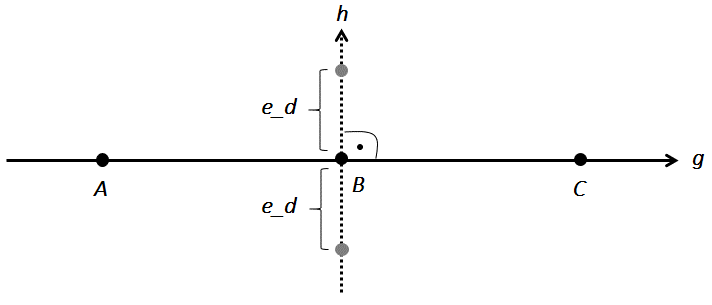
\includegraphics[width=0.5\linewidth]{resources/img/umsetzung/U2/calc_env_point}
    \caption{Bestimmung Spürhüllen}
    \label{fig:real2_envelope_definition_concept}
\end{figure}

Um die Hüll-Punkte für einen Punkt $B$ einer Mittellinie zu bestimmen, wird eine Gerade $g$ durch die
Punkte $A$ und $C$ gelegt, welche sich vor und hinter $B$ befinden.

\begin{ceqn}
\begin{align}
    g: \vec{x} = \overrightarrow{OA} + t \cdot \overrightarrow{AC}
\end{align}
\end{ceqn}

Anschließend wird durch $B$ eine Gerade $h$ gelegt, welche orthogonal zu $g$ verläuft.

\begin{ceqn}
\begin{align}
    h: \vec{x} = \overrightarrow{OB} + t \cdot \hat{X}
\end{align}
\end{ceqn}

Für ihren Richtungsvektor $\hat{X}$, welcher sich aus $\overrightarrow{AC}$ ergibt, gilt
$\overrightarrow{AC} \cdot \hat{X} = 0$. Da $\hat{X}$ ein Einheitsvektor
ist, können die Hüll-Punkte, welche auf $h$ liegen und den Abstand $e_d$ von $B$ besitzten, einfach
bestimmt werden, indem $e_d$ beziehungsweise $-e_d$ für $t$ in die Geradengleichung von $h$ eingesetzt wird.

Auf diese Weise werden die Hüll-Linien für alle Fahrspuren bestimmt. In Abbildung \ref{fig:real2_results_geometry_definition} sind die
Ergebnisse der Spur-Geometrie-Bestimmung dargestellt. Teil a) zeigt die Spurmittellinien mit ihren
sie umgebenden Hüllen. Teil b) zeigt die in die TrackerApplication eingefügten Spuren.

\begin{figure}[H]
    \centering
    \subfloat[]{{
        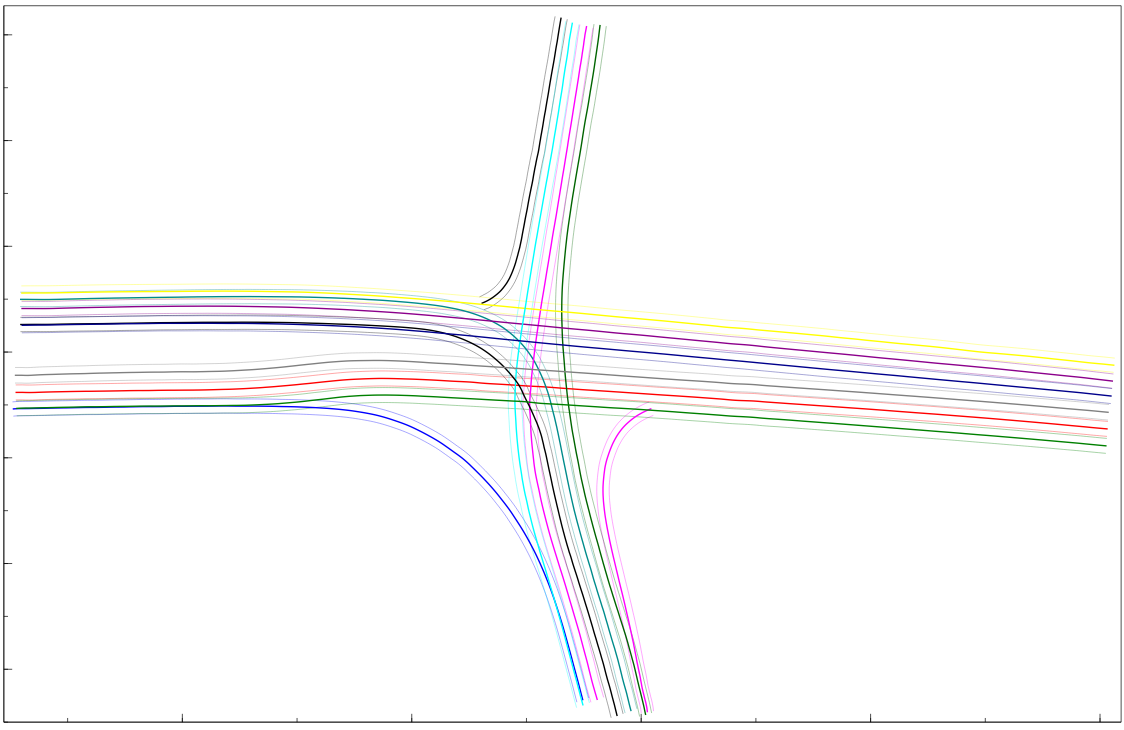
\includegraphics[align=c, width=0.4\linewidth]{resources/img/umsetzung/U2/laneEstimates}
    }}
    \qquad
    \subfloat[]{{
        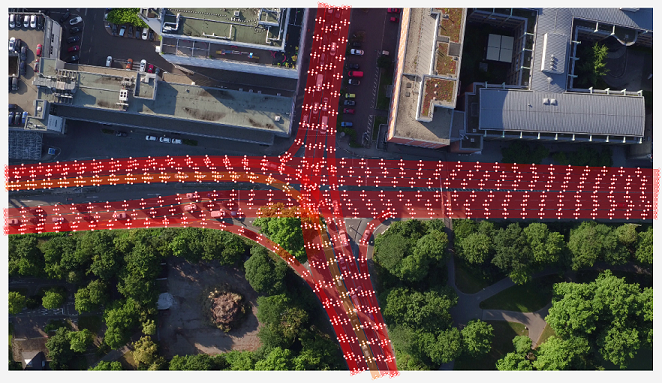
\includegraphics[align=c, width=0.45\linewidth]{resources/img/umsetzung/U2/result_laneEst_Screenshot}
    }}
    \caption{Plot Spurmittellinien und Hüllen a), Ergebnis Spur-Geometrien in TrackerApplication b)}
    \label{fig:real2_results_geometry_definition}
\end{figure}

Die obige Abbildung zeigt, dass die berechneten Spur-Geometrien in den meisten Fällen gut mit den realen
Spur-Dimensionen übereinstimmen. Problematisch sind allerding die Überlagerungen der Spuren in manchen
Regionen. Diese werden im nächsten Schritt entfernt.

\section{Partitionierung von Fahrspuren}
\label{sec:real2_lane_partitioning}

Fahrspuren, welche mithilfe dieser Arbeit erkannt werden, kommen bei der Verkehrsanalyse zum Einsatz.
Unter anderem können mit ihrer Hilfe Spurwechselvorgänge von Fahrzeugen untersucht werden. Damit eine
solche Analyse sinnvoll ist, dürfen sich Fahrspuren nicht über einen größeren Bereich hinweg überlagern.
Aus diesem Grund werden Spuren, welche in Teilen identisch mit anderen verlaufen, partitioniert. Die
identischen Teile werden verworfen und nur die separaten beibehalten.
Unproblematisch ist es, wenn sich Spuren lediglich kreuzen, ihre Überlagerung also geringfügig ist.
In diesem Fall werden die Spuren nicht partitioniert. Es wird daher zwischen sich überlagernden und sich
kreuzenden Spuren unterschieden. Nachfolgend wird das Verfahren
zur Identifikation von sich überlagernden Fahrspuren und der Partitionierungs-Vorgang beschrieben.

Um Fahrspuren zuverlässig und sinnvoll partitionieren zu können, müssen grundlegend zwei Probleme bewältigt
werden. Es müssen zuerst die sich überlagernden Spur-Paare und deren Schnittpunkte gefunden werden und
anschließend muss für jedes Paar entschieden werden, welche Spur partitioniert wird und welche erhalten bleibt.
Hierzu wird zuerst die Menge der Spur-Geometrien in drei Kategorien unterteilt:

\begin{itemize}
    \item isolierte Fahrspuren
    \item primäre Fahrspuren
    \item sekundäre Fahrspuren
\end{itemize}

Isolierte Fahrspuren sind hierbei jene, welche keine Überschneidung mit anderen Spuren besitzen. Primäre
Fahrspuren besitzen keine Überschneidungen untereinander, können sich aber mit anderen Spuren kreuzen oder
von ihnen überlagert werden. In einer Menge von Spur-Geometrien bildet das größte Subset von parallel
zueinander verlaufenden Spuren die primären Spuren. Sekundäre Fahrspuren sind all jene, welche
weder isoliert noch primär sind. In Abbildung \ref{fig:real2_prim_and_sec_lanes} a) sind die primären und
sekundären Spur-Geometrien der Neckartor-Kreuzung dargestellt.

\begin{figure}[H]
    \centering
    \subfloat[]{{
        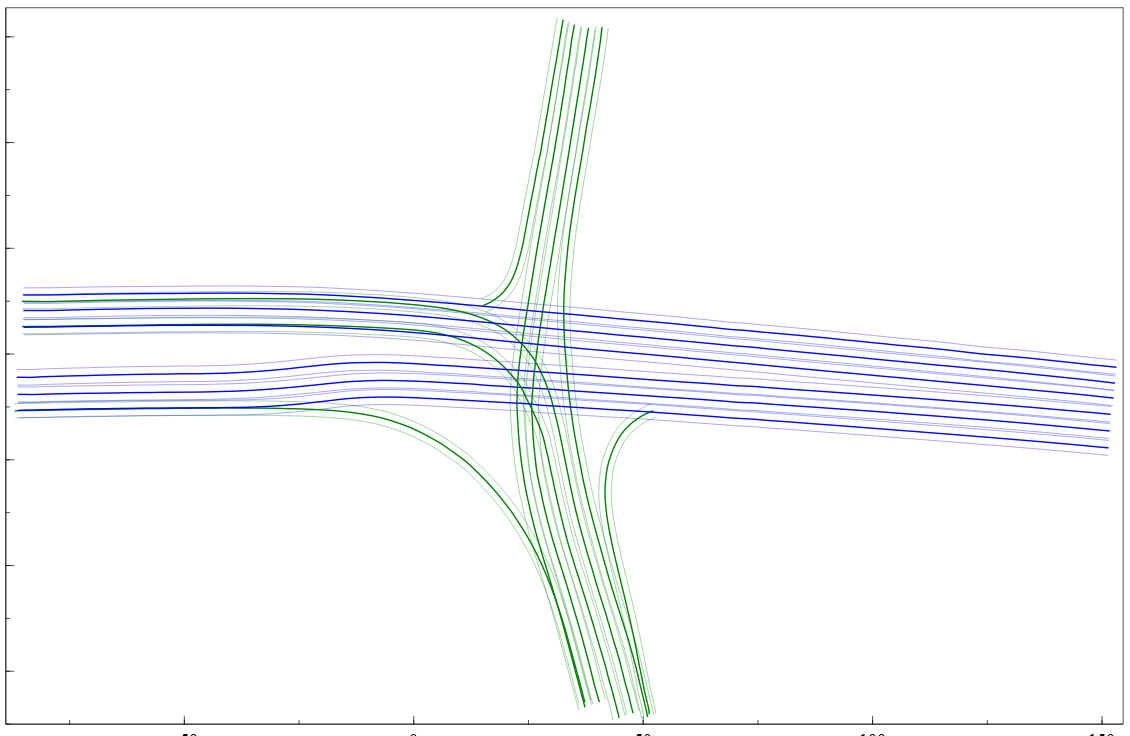
\includegraphics[align=c, width=0.35\linewidth]{resources/img/umsetzung/U2/prims_and_secs}
    }}
    \qquad
    \subfloat[]{{
        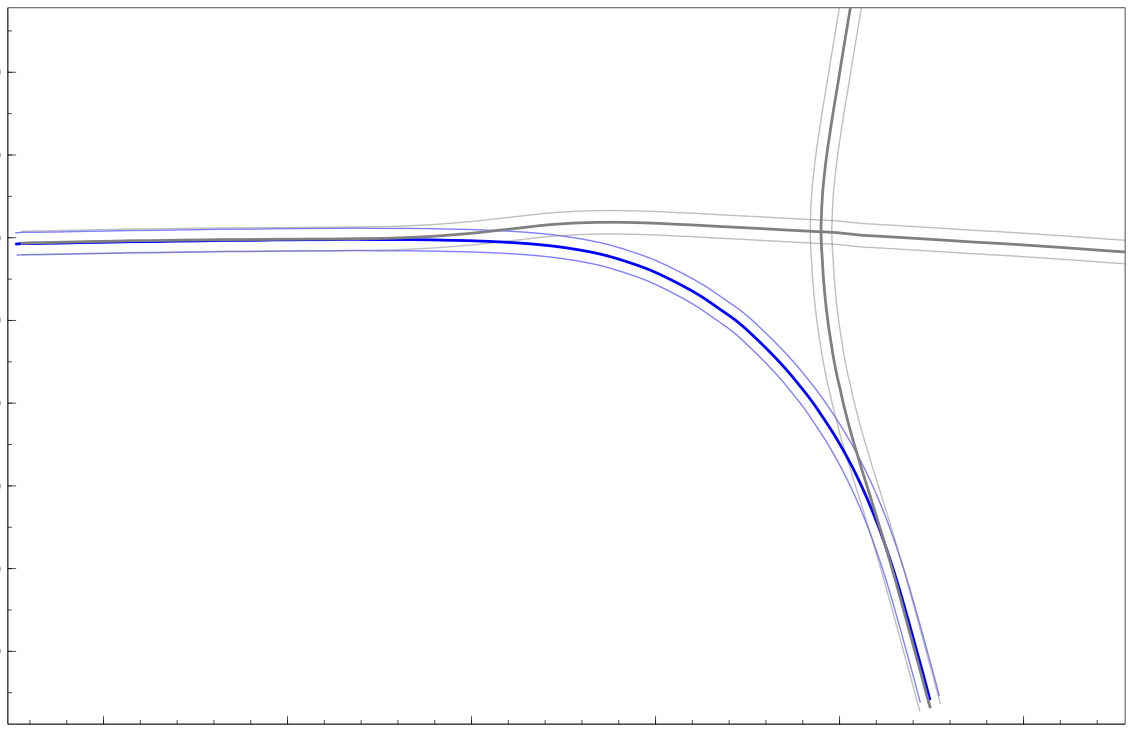
\includegraphics[align=c, width=0.35\linewidth]{resources/img/umsetzung/U2/overlapping_lanes}
    }}
    \caption{a) Primäre (blau) und sekundäre (grün) Spuren, b) sich überlagernde und kreuzende Spur-Paare}
    \label{fig:real2_prim_and_sec_lanes}
\end{figure}

Nachdem die Spuren, anhand der oberen Definition, in die drei Kategorien unterteilt wurden, werden
anschließend die primären und sekundären Spuren nach sich überlagernden Paaren durchsucht.
Zwei Spuren überschneiden sich, wenn, wie in
Abbildung \ref{fig:real2_lane_crossing} zu sehen, die Mittellinie einer Spur innerhalb der Hülle einer
anderen Spur liegt. Die Punkte $b_1$ und $b_2$ entsprechen hierbei den äußeren und inneren Grenzpunkten
der Überschneidung der Mittellinie von $l_2$ mit der Hülle von $l_1$. Zur Bestimmung der Schnittmenge
wird wieder die JTS Topology Suite eingesetzt.

\begin{figure}[H]
    \centering
    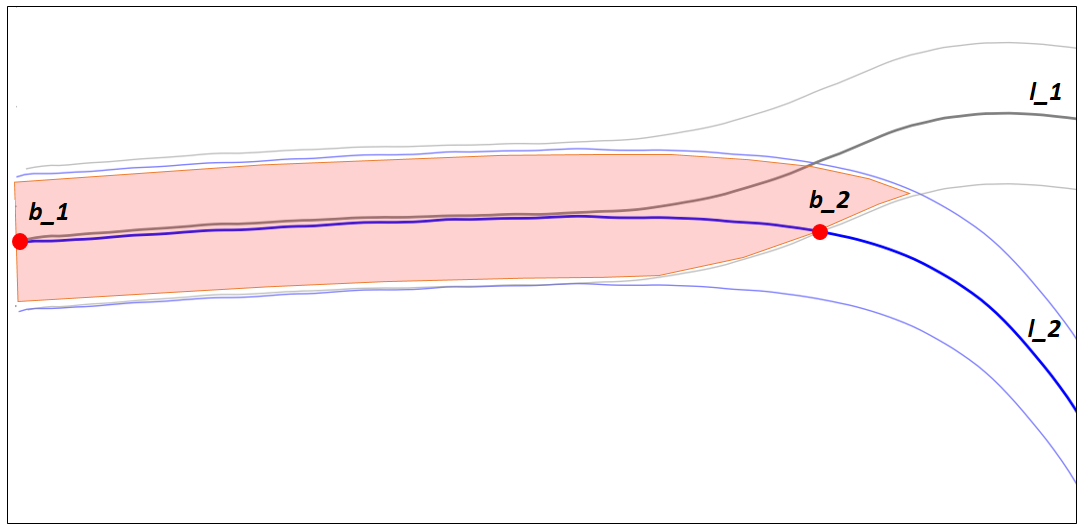
\includegraphics[width=0.5\linewidth]{resources/img/umsetzung/U2/lane_crossing}
    \caption{Überlagerung zweier Spur-Abschnitte}
    \label{fig:real2_lane_crossing}
\end{figure}

Zwei Spuren $l_1$ und $l_2$ kreuzen sich nicht nur, sondern überlagern sich, wenn der Abschnitt zwischen
den Grenzpunkten $b_1$ und $b_2$ mindestens 10\% der Spurlänge ausmacht. Auf diese Weise werden die
sich überlagernden Spur-Paare und die zugehörigen Schnittpunkte bestimmt.
Aus jeder Überschneidung ergeben sich zwei Spur-Paare.
Im Fall von Abbildung \ref{fig:real2_lane_crossing} wird einerseits $l_1$ von $l_2$ überlagert und andererseits
$l_2$ von $l_1$.
Daher enthält Abbildung \ref{fig:real2_prim_and_sec_lanes} b) beispielsweise vier sich überlagernde Spur-Paare
(blau-grau) und zwei sich kreuzende Paare (grau-grau).

Nachdem auf die oben beschriebene Weise die sich überlagernden Spur-Paare bestimmt wurden, wird anschließend
entschieden, welche Spur der Paare partitioniert wird und welche erhalten bleibt. Zuerst wird hierzu
überprüft, ob es sich bei einer der Geometrien um eine primäre Fahrspur handelt. Ist dies der Fall, so
bleibt diese vollständig. Existiert in einem Paar keine primäre Spur, so wird das Krümmungsverhalten der Spuren
um ihren Schnittpunkt herum untersucht. Das Ziel ist es, jene Spur, welche eine stärker Krümmung besitzt,
zu partitionieren. Es handelt sich bei ihr mit höherer Wahrscheinlichkeit um eine Abbiegespur et cetera,
welche aus einer geraden Spur hervorgeht oder in eine solche übergeht. Der Algorithmus zur Auswahl
der gekrümmteren Spur ist in Listing \ref{lst:pseudo_selectMoreCurvy} beschrieben.
\begin{lstlisting}[caption=Pseudocode Auswahl gekrümmtr Fahrspur, language=Pseudo, label=lst:pseudo_selectMoreCurvy]
algorithm selectMoreCurvyLane:
  input:  lane-geo: l1, lane-geo: l2, boundPoints: bounds
  output: l1 or l2 based on curviness around bounds

  innerBoundPoint := select inner bound point based on distance
                     from b1 and b2 to the edges of l1

  l1Subset := get subset of l1 around innerBoundPoint (length 15 points)
  l2Subset := get subset of l2 around innerBoundPoint (length 15 points)

  l1SubCurvMea := estimate curvature of l1Subset
  l2SubCurvMea := estimate curvature of l2Subset

  if l1SubCurvMea >= l2SubCurvMea then
    return l1
  else
    return l2
  end
\end{lstlisting}

Im Fall der sich überlagernden Spurpaare in Abbildung \ref{fig:real2_lane_crossing} ist $b_2$ der \textit{innerBoundPoint}.
Zur Bestimmung der Krümmung einer Fahrspur in einem Bereich, siehe Listing \ref{lst:pseudo_selectMoreCurvy}
Zeile 8 + 9, wird der Winkel $\varphi$ zwischen den Richtungsvektoren des Anfang und Endes der Teilspur berechnet.
Er ergibt sich anhand Gleichung \ref{eq_angle_skalar}.
Unterscheidet sich die Krümmung der zwei Spuren im Bereich ihrer Überschneidung nur geringfügig, so wird
die kürzere Spur partitioniert.

\begin{ceqn}
\begin{align}
\label{eq_angle_skalar}
    \varphi=\arccos \frac{\vec a \cdot \vec b}{|\vec a| |\vec b|}
\end{align}
\end{ceqn}

Nachdem alle zu teilenden Spuren und die zugehörigen Grenzpunkte
bestimmt wurden, folgt die eigentliche Partitionierung. Aus den Spur-Geometrien werden alle Bereiche
entfernt, welche zwischen den zwei Grenzpunkten einer Überlagerung liegen. In Abbildung \ref{fig:real2_lane_crossing}
wird so beispielsweise der rot gekennzeichnete Bereich der Spur $l_2$ zwischen $b_1$ und $b_2$ entfernt.

Abbildung \ref{fig:real2_results_partitioning} zeigt das Ergebnis der Spur-Partitionierung im Fall des
Neckartor Datensatzes. Es wurden alle Spur-Überlagerungen entfernt.

\begin{figure}[H]
    \centering
    \subfloat[]{{
        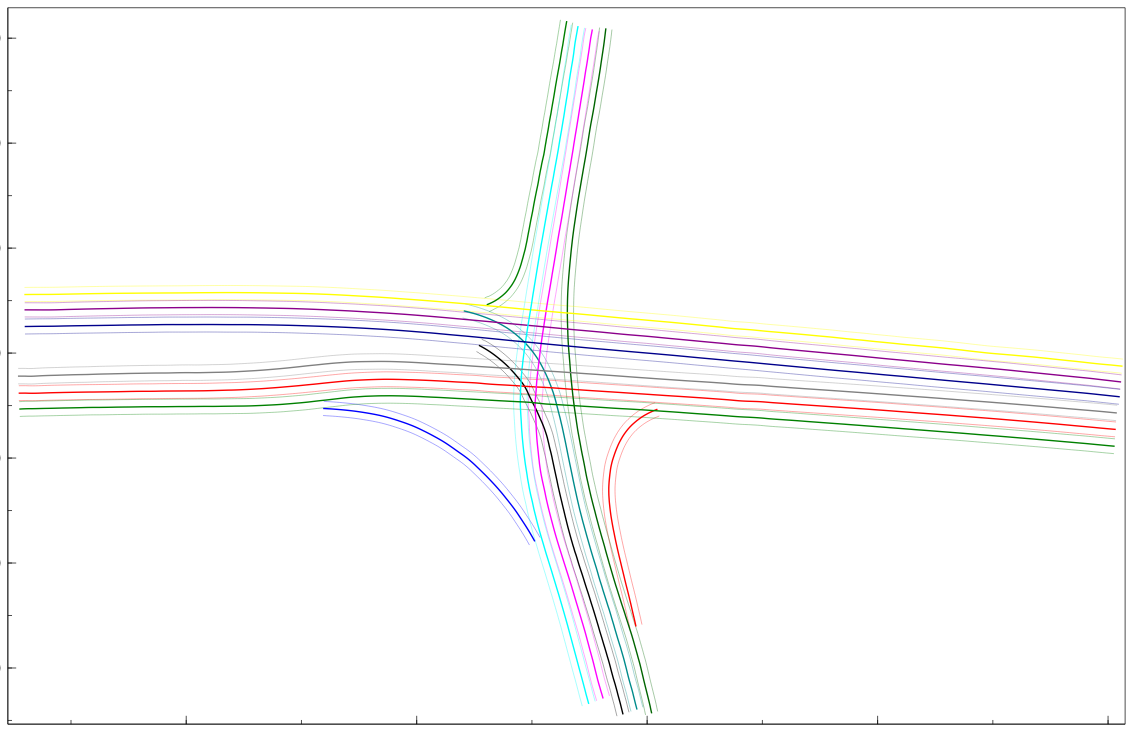
\includegraphics[align=c, width=0.4\linewidth]{resources/img/umsetzung/U2/partitionedLanes}
    }}
    \qquad
    \subfloat[]{{
        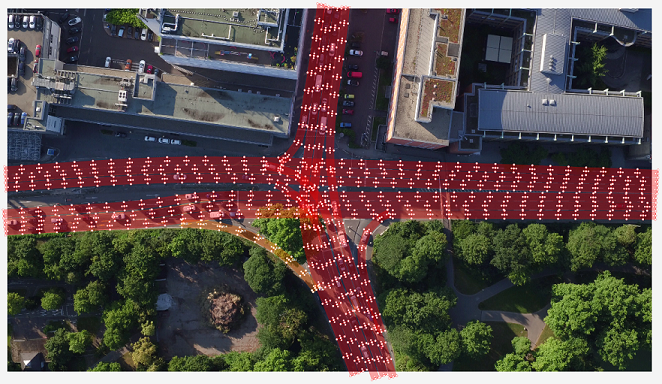
\includegraphics[align=c, width=0.45\linewidth]{resources/img/umsetzung/U2/result_lanePartitioned_Screenshot}
    }}
    \caption{Plot partitionierte Spur-Geometrien a), Ergebnis in der TrackerApplication b)}
    \label{fig:real2_results_partitioning}
\end{figure}

Die so ermittelten Spur-Geometrien entsprechen in den meisten Fällen bereits dem gewünschten Ergebnis,
da sie die realen Fahrspur-Verläufe gut wiederspiegeln und keine Überlagerungen mehr existieren.
In einigen Szenarien kann es jedoch vorkommen, dass nach der Geometrie-Ermittlung und der Partitionierung
die Fahrspur-Geometrien die reale Straßen-Topologie noch nicht korrekt abbilden. Aus diesem Grund werden die
Spur-Geometrien in einem finalen Schritt nochmals optimiert.

\section{Optimierung der Spur-Geometrien}

Die nach dem Partitionierungs-Schritt vorliegenden Spur-Geometrien besitzen in einigen Fällen noch Defekte.
Das am häufigsten auftretende Problem ist, dass die Spur-Geometrien nicht breit genug sind.
Abbildung \ref{fig:real2_pre_opt} zeigt beispielsweise die Spur-Geometrien eines Straßen-Abschnitts,
in welchem sich zu Beginn zwei parallele Fahrspuren befinden, welche sich am Ende in vier Spuren aufteilen.
Es ist erkennbar, dass die zwei Fahrspuren zu Beginn nicht direkt aneinander angrenzen
und daher in diesem Abschnitt nicht breit genug sind. In diesem Fall resultiert die zu niedrige Fahrbahnbreite
aus der starken Überlagerung der vier Spur-Geometrien zu Beginn, was eine falsche Schätzung der Spur-Breite verursacht
(siehe Abschnitt \ref{sec:real2_define_lane_envelope}).

\begin{figure}[H]
    \centering
    \fbox{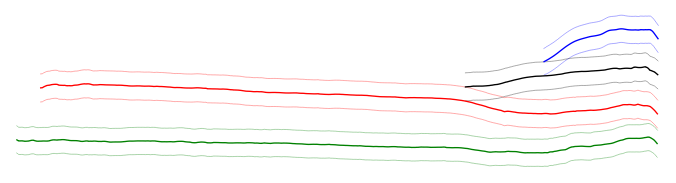
\includegraphics[align=c, width=0.7\linewidth]{resources/img/umsetzung/U2/laneOpt_partitioned_pre}}
    \caption{Beispiel zu schmale Spur-Geometrien}
    \label{fig:real2_pre_opt}
\end{figure}

Um Effekte wie diesen zu korrigieren, werden nach der Partitionierung nun nochmals die Breiten aller Spur-Geometrien
neu bestimmt. Im Gegensatz zu dem verwendeten Vorgehen aus Abschnitt \ref{sec:real2_define_lane_envelope},
bei welchem für jede Spur eine feste Breite berechnet wurde, wird diese nun für jeden Punkt der Spur einzelt
berechnet. Hierdurch wird es möglich, dass beispielsweise die schwarze und grüne Spur aus Abbildung \ref{fig:real2_pre_opt}
zu Beginn breiter sind, als an ihrem Ende.

Der zur Bestimmung der neuen Spur-Breiten eingesetzte Algorithmus hat vereinfacht gesehen den nachfolgenden Ablauf:

\begin{itemize}
    \item Wähle eine Spur-Geometrie $l$
    \item Für jeden Punkt $p$ der Mittellinie von $l$ mit Position $i$:
    \begin{itemize}
        \item Suche korrespondierende Punkte $P_k = \{pk_0\ ...\ pk_n\}$ auf benachbarten Spuren
        \item Wähle einen benachbarten Punkt $pk_j \in P_k$
        \item Verwende die Distanz zwischen $p$ und $pk_j$ als Spurbreite von $l$ an Position $i$
    \end{itemize}
\end{itemize}

Entscheidend bei diesem Verfahren ist es, den richtigen Punkt $pk_j$ auszuwählen. Dieser muss grundsätzlich
auf jener Spur liegen, welche im Bereich des Punktes $p$ parallel zu $l$ verläuft und ihr am nächsten liegt.

Nachdem auf diese Weise für eine Spur punktweise die neuen Breiten bestimmt wurden, werden diese noch mithilfe
eines gleitenden Mittelwert Verfahrens geglättet. Anschließend werden neue Spurhüllen, mittels dem in
Abschnitt \ref{sec:real2_create_envelopes} vorgestellten Vorgehen, erzeugt.
Das Ergebnis der Geometrie-Optimierung für den Fall der in Abbildung \ref{fig:real2_pre_opt} enthaltenen Spuren,
ist nachfolgend dargestellt.

\begin{figure}[H]
    \centering
    \fbox{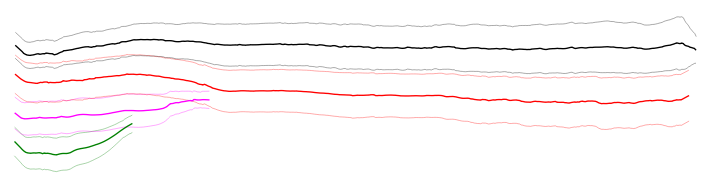
\includegraphics[align=c, width=0.7\linewidth]{resources/img/umsetzung/U2/laneOpt_optimized}}
    \caption{Beispiel zu schmale Spur-Geometrien}
    \label{fig:real2_pre_opt}
\end{figure}

Die Fahrspur-Erkennung ist nach dem Optimierungs-Schritt abgeschlossen. Die aus den Trajektorie-Daten
extrahierten Spur-Geometrien stimmen in den meisten Fällen mit den realen Fahrbahnverläufen überein.
Die Stärken und Schwächen des entwickelten Algorithmus werden im nachfolgenden Auswertungskapitel nochmals
zusammengefasst und ausgewertet.